\chapter{OVERVIEW OF PROPOSED METHOD} 

\begin{figure}
\centering
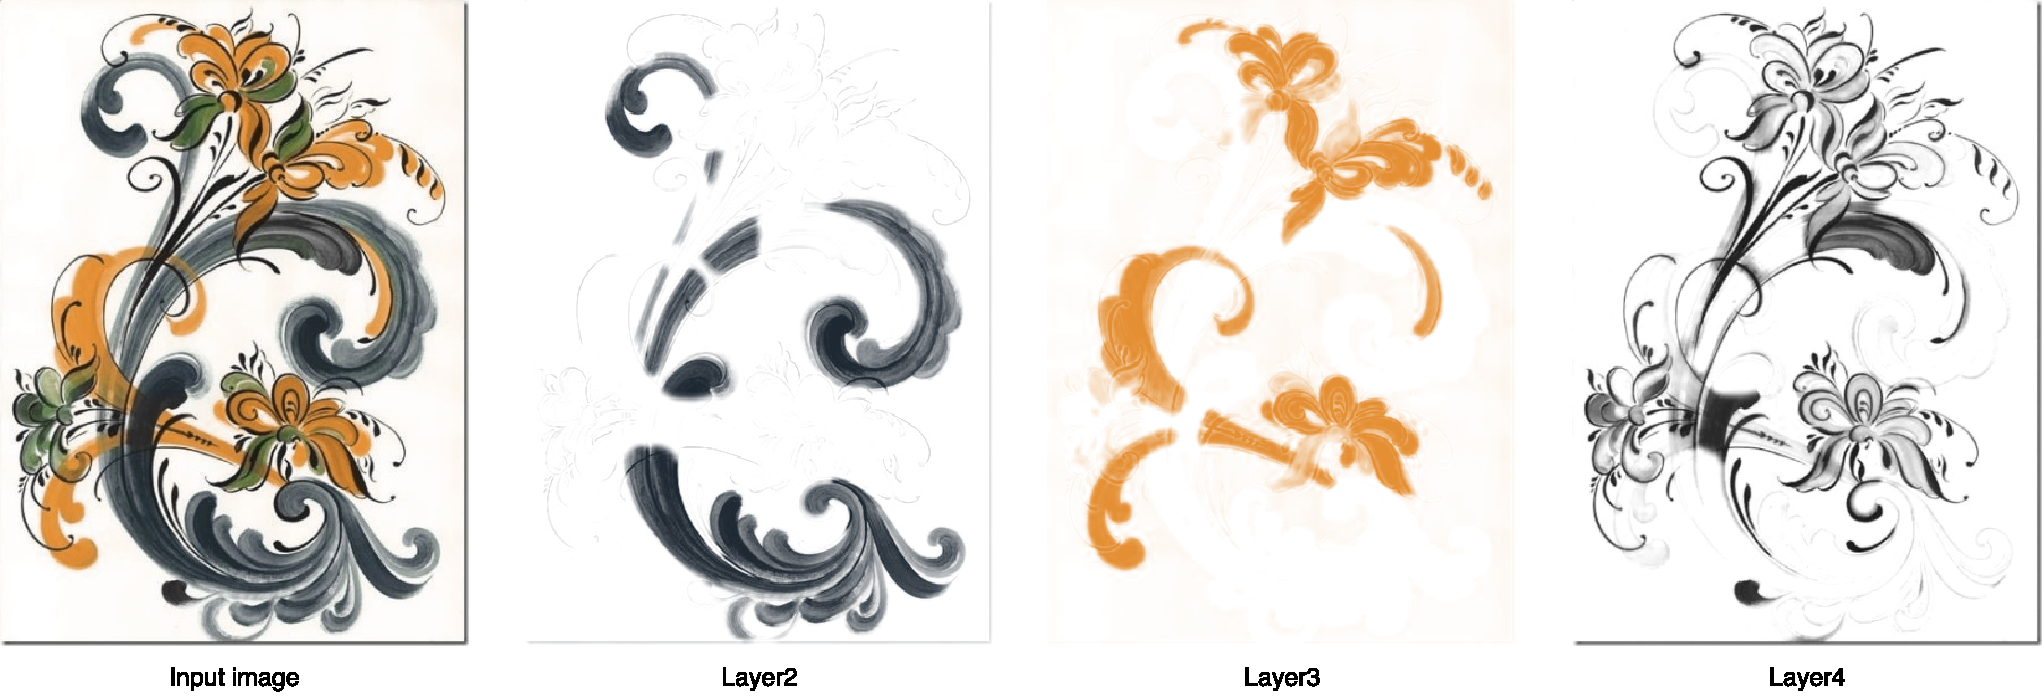
\includegraphics[height=0.2\textheight]{layers.pdf}
\caption{Decomposition layers }
\label{decom:4layers}
\end{figure}
As shown in Figure \ref{decom:4layers}, a given painting is firstly decomposed into a set of layers in terms of RGB values. Secondly, each resulting layer is further segmented into multiple regions which represent brush strokes respectively. Thirdly, the depth map of each brush stroke is generated by the shape from shading technique	s individually. After that, the desired bas-relief is generated by merging all the depth maps of brush strokes together.
\newline
The key point is to extract brush strokes from input paintings. Overlapped strokes make colors blend. To deal with it, layer decomposition is firstly employed here, which decomposes the painting into a set of single colored and translucent layers. In brush paintings, each stroke only utilizes a single palette color. Therefore, layer decomposition helps classify brush strokes separately into different layers based on the palette color so that every layer contains the strokes which are well separated.
However, wrong layer decomposition may cut one stroke into two or more layers. It is observed that typically strokes of such paintings follow regular patterns. For instance, Rosemaling paintings employ many C and S strokes, and the color and transparency change very little in the direction of the stroke. We introduce the edge tangent flow (ETF) field and the coherent line \cite{kang2007coherent} to enhance such features in paintings, which is in favor of preserving the wholeness of the strokes in every layer and effectively avoid wrong layer decomposition.
\newline
The coherent line is further involved in the MSERs algorithm \cite{donoser2006efficient} again for extracting spurious edges within one layer.
Furthermore, to generate the depth maps of the strokes individually, we perform shape from shading on the opacity of the paintings instead of the intensity her	e, since the opacity has a bigger range than the intensity (as can be seen in Figure \ref{histo} for detail). SFS techniques may generate details of surfaces in terms of image texture. It is desirable to transfer the features of the paintings, e.g. the density of colors, to the surface of the brush stroke models.
\newline
The depth maps of all the strokes are then merged together to form the desired bas-relief. We hope to point out that the employed orthographic SFS technique tends to encourage interior growth within a closed region due to the Eikonal Equation, which may result in the growth of a background region surrounded by strokes. In general, the background plane should be unchanged. Thus, generating strokes individually not only benefits the composition of bas-reliefs but also avoid this technique issue.
Moreover, the stroke order and shape may be edited by users to cater for the request of recomposition in art design. The user may recompose the stroke models in 3D space for secondary creation.
\newpage 